\documentclass{article}\usepackage[]{graphicx}\usepackage[]{color}
% maxwidth is the original width if it is less than linewidth
% otherwise use linewidth (to make sure the graphics do not exceed the margin)
\makeatletter
\def\maxwidth{ %
  \ifdim\Gin@nat@width>\linewidth
    \linewidth
  \else
    \Gin@nat@width
  \fi
}
\makeatother

\definecolor{fgcolor}{rgb}{0.345, 0.345, 0.345}
\newcommand{\hlnum}[1]{\textcolor[rgb]{0.686,0.059,0.569}{#1}}%
\newcommand{\hlstr}[1]{\textcolor[rgb]{0.192,0.494,0.8}{#1}}%
\newcommand{\hlcom}[1]{\textcolor[rgb]{0.678,0.584,0.686}{\textit{#1}}}%
\newcommand{\hlopt}[1]{\textcolor[rgb]{0,0,0}{#1}}%
\newcommand{\hlstd}[1]{\textcolor[rgb]{0.345,0.345,0.345}{#1}}%
\newcommand{\hlkwa}[1]{\textcolor[rgb]{0.161,0.373,0.58}{\textbf{#1}}}%
\newcommand{\hlkwb}[1]{\textcolor[rgb]{0.69,0.353,0.396}{#1}}%
\newcommand{\hlkwc}[1]{\textcolor[rgb]{0.333,0.667,0.333}{#1}}%
\newcommand{\hlkwd}[1]{\textcolor[rgb]{0.737,0.353,0.396}{\textbf{#1}}}%
\let\hlipl\hlkwb

\usepackage{framed}
\makeatletter
\newenvironment{kframe}{%
 \def\at@end@of@kframe{}%
 \ifinner\ifhmode%
  \def\at@end@of@kframe{\end{minipage}}%
  \begin{minipage}{\columnwidth}%
 \fi\fi%
 \def\FrameCommand##1{\hskip\@totalleftmargin \hskip-\fboxsep
 \colorbox{shadecolor}{##1}\hskip-\fboxsep
     % There is no \\@totalrightmargin, so:
     \hskip-\linewidth \hskip-\@totalleftmargin \hskip\columnwidth}%
 \MakeFramed {\advance\hsize-\width
   \@totalleftmargin\z@ \linewidth\hsize
   \@setminipage}}%
 {\par\unskip\endMakeFramed%
 \at@end@of@kframe}
\makeatother

\definecolor{shadecolor}{rgb}{.97, .97, .97}
\definecolor{messagecolor}{rgb}{0, 0, 0}
\definecolor{warningcolor}{rgb}{1, 0, 1}
\definecolor{errorcolor}{rgb}{1, 0, 0}
\newenvironment{knitrout}{}{} % an empty environment to be redefined in TeX

\usepackage{alltt}[11pt]
%Required: You must have these
\usepackage{graphicx}
\usepackage{tabularx}
\usepackage{natbib}

\usepackage{array}
\usepackage{amsmath}
%\usepackage[backend=bibtex]{biblatex}
\setkeys{Gin}{width=0.8\textwidth}
%\setlength{\captionmargin}{30pt}
\setlength{\abovecaptionskip}{10pt}
\setlength{\belowcaptionskip}{10pt}
\topmargin -1.5cm 
\oddsidemargin -0.04cm 
\evensidemargin -0.04cm 
\textwidth 16.59cm
\textheight 23.94cm 
\parskip 7.2pt 
\renewcommand{\baselinestretch}{1.2} 	
\parindent 0pt


\bibliographystyle{..//refs/styles/besjournals.bst}
%\usepackage{xr-hyper}
\usepackage{hyperref}
\title{Aridity and floral architecture drive hysteranthous flowering in the North American cherries (\textit{Prunus spp.})}
\IfFileExists{upquote.sty}{\usepackage{upquote}}{}
\begin{document}
\maketitle


\section*{Introduction}
\noindent Woody perennials have a unique ability among plants to seasonally begin reproduction prior to vegetative growth \citep{}. This flowering-first phenological sequence known as hysteranthy, proteranthy or precocious flowering is particularly common in temperate forests around the globe \citep{}. A number of studies suggest that this flower-leaf sequences (FLSs) are under selection, and that flowering first has functional significance \citep{}.

\noindent The most common, and well-tested explanation for the evolution of hysteranthy is that it is adaptive for wind-pollination as leafless canopies increase wind speeds for pollen transport and reduce the likelihood of pollen interception on vegetation \citep{}. However, this hypothesis fails to address the prevalence of hysteranthous taxa that are biotically-pollinated. Approximately 30\% of species of Eastern temperate forests of North America flower before leafing out, and of those, approximately 20\% are biotically pollinated  \citep{}. Despite the pervasiveness of this phenological syndrome, direct tests of the function of hysteranthy in biotically pollinated taxa are exceedingly rare.

\noindent Yet, based on decades of natural history accounts of hysteranthous species around th globe, we have identified two major hypotheses regarding the function of hysteranthy in biotically-pollinated taxa. Each hypothesis makes logical predictions about how hysteranthous flowering should other plant traits should co-vary, and these hypotheses and their predictions can be used to guide further inquiry into the adaptive significance of hysteranthy.

The \textbf{water dynamics hypothesis} suggests that hysteranthy is an adaptation to arid environments, allowing for plant to partition the hydraulic demand of hydrated flowers and transpiring leaves across the growing season \citep{}. If this is the case, this hypothesis predicts that hysteranthous species should be more commonly found in dry environments.  

The \textbf{pollinator visibility hypothesis} suggests that hysteranthy is an adaptation to attract visually-foraging pollinators \citep{}. If this is the case, this hypothesis predicts that hysteranthous species may invest less in other floral traits for pollinator attraction such as size of floral display or chemical attraction. 

\noindent Still others have suggested that hysteranthy is simply the by-product of selection for early flowering \citep{},and that variation in flower-leaf sequences among species is driven by developmental, physical or phylogenetic constraints than adaptive selection \citep{}. However, even this null hypothesis make testable predictions. If this is the case, hysteranthy should co-vary with other early-flowering associated traits like long fruit development periods or large fruit sizes \citep{} and the phylogenetic signal for hysteranthy should be strong.

\noindent With mounting evidence that climate driven shifts in phenological phases are altering the duration and order of flower-leaf sequences \citep{} understanding the functional significance of hysteranthy is vital to forecasting the demography and performance of forest communities in an era of global climate change. However, there are two major methodological challenges to testing these hypotheses:

\noindent First, characteristics like aridity tolerance, pollinator attraction, and reproductive investment are the emergent product of a suite of biological traits \citep{}. Thus, when analyzing selective drivers of any particular trait at large taxonomic scales, unmeasured trait differences may obscure the estimated effects of the trait of interest, biasing results. %For example, hysteranthy may contribute significantly to differences in aridity tolerance between two species with similar root architecture, leaf characteristics and xylem anatomy, but matter much less when comparing deep rooted species to shallow rooted ones. 
This is a common problem in trait-based ecology, and one of the most promising solutions for understanding the functional significance of hysteranthy in woody plants is through character deconstruction \citep{}; comparing flower-leaf sequences variation for only a subset of taxa of shared phylogenetic and morphological character.   

\noindent The second challenge for robust testing of hysteranthy hypotheses is that most characterizations of flower-leaf phenological sequences are based on expert-opinion verbal descriptions(e.g. ``flowers before leaves" or ``flower before/with leaves"), which make comparisons across taxa, time and space difficult sensitive to observer bias (see, \citep{}). 

\noindent This problem can be overcome by adopting standardized quantitative measures of plant phenology for observational studies and applying them to historic data records. Herbarium records are an excellent source of data that can be leveraged for quantitative phenological measurements \citep{}, but have not be used widely to investigate variability of flower-leaf sequences variation among and within species.

\noindent In this study, we combine a large data set of occurrence records with published descriptions of flower-leaf sequences and plant traits for North American species in the genus \textit{Prunus} to test the predicted associations of the major hysteranthy hypotheses at the genus level. We then further deconstruct patterns of flower-leaf sequences % help here




%<<>>=
%mich.data<-read.csv("..//..//sub_projs/MTSV_USFS/michdata_final.csv")
%table(mich.data$pro2,mich.data$Pollination)

%table(mich.data$pro)
%42/147
%table(mich.data$pro2)
%82/147

@



%Generally speaking, hysteranthy is unique and common in temperate forest. Seems functionial. The most common, and well tested, explaination is that is hysteranthy evolved for wind-pollination. However that doesn't explain its prevalence in biotically pollinated taxa. Quote some statistic based new phyt paper. Tests of the function on hysteranthy in biotically pollinated taxa are exceedingly rare in the literature,, but may be critial for predicting species responses to global change.

%While direct tests are limited, investegation of hysteranthy beneifit from a rich theoretical literature and several hypotheses have emerge.

%Review them briefly and make predictions
%\begin{enumerate}
%\item Drought adaptation: (could be plastic or selected) aridity in range
%\item insect visaibility: floral morphology
%\item Null functionality early flowering. Fruit size or phenology
%\item Phylogeny may also matter
%\end{enumerate}

%While each hypothesis generates testible predictions there are several methodological challenges.
%\begin{enumerate}
%\item Unmeasured species difference compensate for measure traits
%\item data quality based on expert opinion
%\end{enumerate}

%These issues could be over come with:
%\begin{enumerate}
%\item character deconstruction
%\item detailed quantitative measurements of flower leaf sequence phenology
%\end{enumerate}

%We do this:
%\begin{enumerate}
%\item Coarse analyses of the flower-leaf sequences of North American \textit{Prunus} species and their hypothesis relevant traits based on published data
%\item Higher resolution inquiry of the fLower-leaf sequences and associated character traits based on our own measurements from a century worth of herbaria samples on a section of the Prunus subgenus Prunocerasus the American plums
%\end{enumerate}

\section*{Methods}
\subsection{Study system}
\noindent The genus \texit{Prunus} comprises approximately 200 species distributed across the globe \citep{}. Of 40-50 species native to or naturalized in North America, \textit{Prunus}species display the full spectrum of variation in flower-leaf sequences \citep{} and show marked inter-specific variation in habitat requirements and functional traits making them an ideal system in which to investigate the inter-relationship between hysteranthy and traits predicted by the two major hysteranthy hypotheses.

\noindent Within the genus, The American plums (\textit{Prunus} subsp. \textit{Prunus} sect. \textit{Prunocerasus}) offer potential for an additional, higher resolution investigation of drivers of hysteranthous flowering. Like the genus at large, the 16 species that make up the section are distributed across North America and show pronounced inter-specific variation in flower leaf sequences. While within the larger genus species can be separated into three distinct morphological clades by inflorescence architecture (solitary, corymbose or racemose) all members of the section have solitary inflorescences \citep{} allowing for even more refined character deconstruction. Species in this section are well represented in herbaria records, making them a tractable group to measure and assess intra-specific variation in flower-leaf sequences as well as other ecological and morphological characteristics related to the hysteranthy hypotheses described above. 


\subsection{Genus level analyses}
Data source\\
Methods for analysis\\

\subsection{Section level analyes}
Methods for herbaria measurements\\
Methods for analysis\\
\pagebreak

\section*{Results}
\subsection*{Drivers of hysteranthy in\textit{Prunus spp.} of North America}
Likelihood of hysteranthy was associated increasing aridity, flowering and inflorescence size and their interaction. Fruit size had little effect of the likelihood of hysteranthy and at the genus level, the phylogenetic signal in hysteranthy was X suggesting weak to moderate phylogeny structure.


\subsection*{Drivers of hysteranthy in sect. \textit{Prunocerasus} }
Within the section \textit{Prunocerasus}, hysteranthy was associated with smaller fruit (). There was no relationship between flower size, fruit phenology, or mean pdsi and the phylogenetic signal of hysteranthy was virtually non-existent within this sub-clade. WHen we investigated

\section*{Discussion}
At the genus level we identified a strong negative relationship between the likelihood a species is hysteranthous and flower size, inflorescence size and aridity (). Fruit size appeared to have little influence on hysteranthy () and the phylogenetic signal for in the evolution of flower-leaf sequences was weak-moderate ().
By contrast, with in the section of \text{Prunocerasus}, fruit size was the only trait significantly associated with increased likelihood relationship, though our estimated effect was relatively weak, and of note the positive relationship between fruit size and FLS catagory (suggestion that hysteranthy is associated with smaller fruit), is counter to the expectation about the relationship between fruit size and flowering time\ \citep{}.




\secction Floral display in hysteranthy 

Two possible explanations. Data type. Taxonomic scale. 

There will probably be things about taxonomic scale. Ie attraction showing up at the genus but not section level. Major discussion of why. \\
Pollinator attraction and drought tolerance are a suite of traits and we only measured one axis of them and even with character deconstruction this could matter\\
Mechanistic experiments would still be useful, ie does water limitation influence FLS plasticity
\newpage
\section*{Figures}
    \begin{figure}[h!]
    \centering
 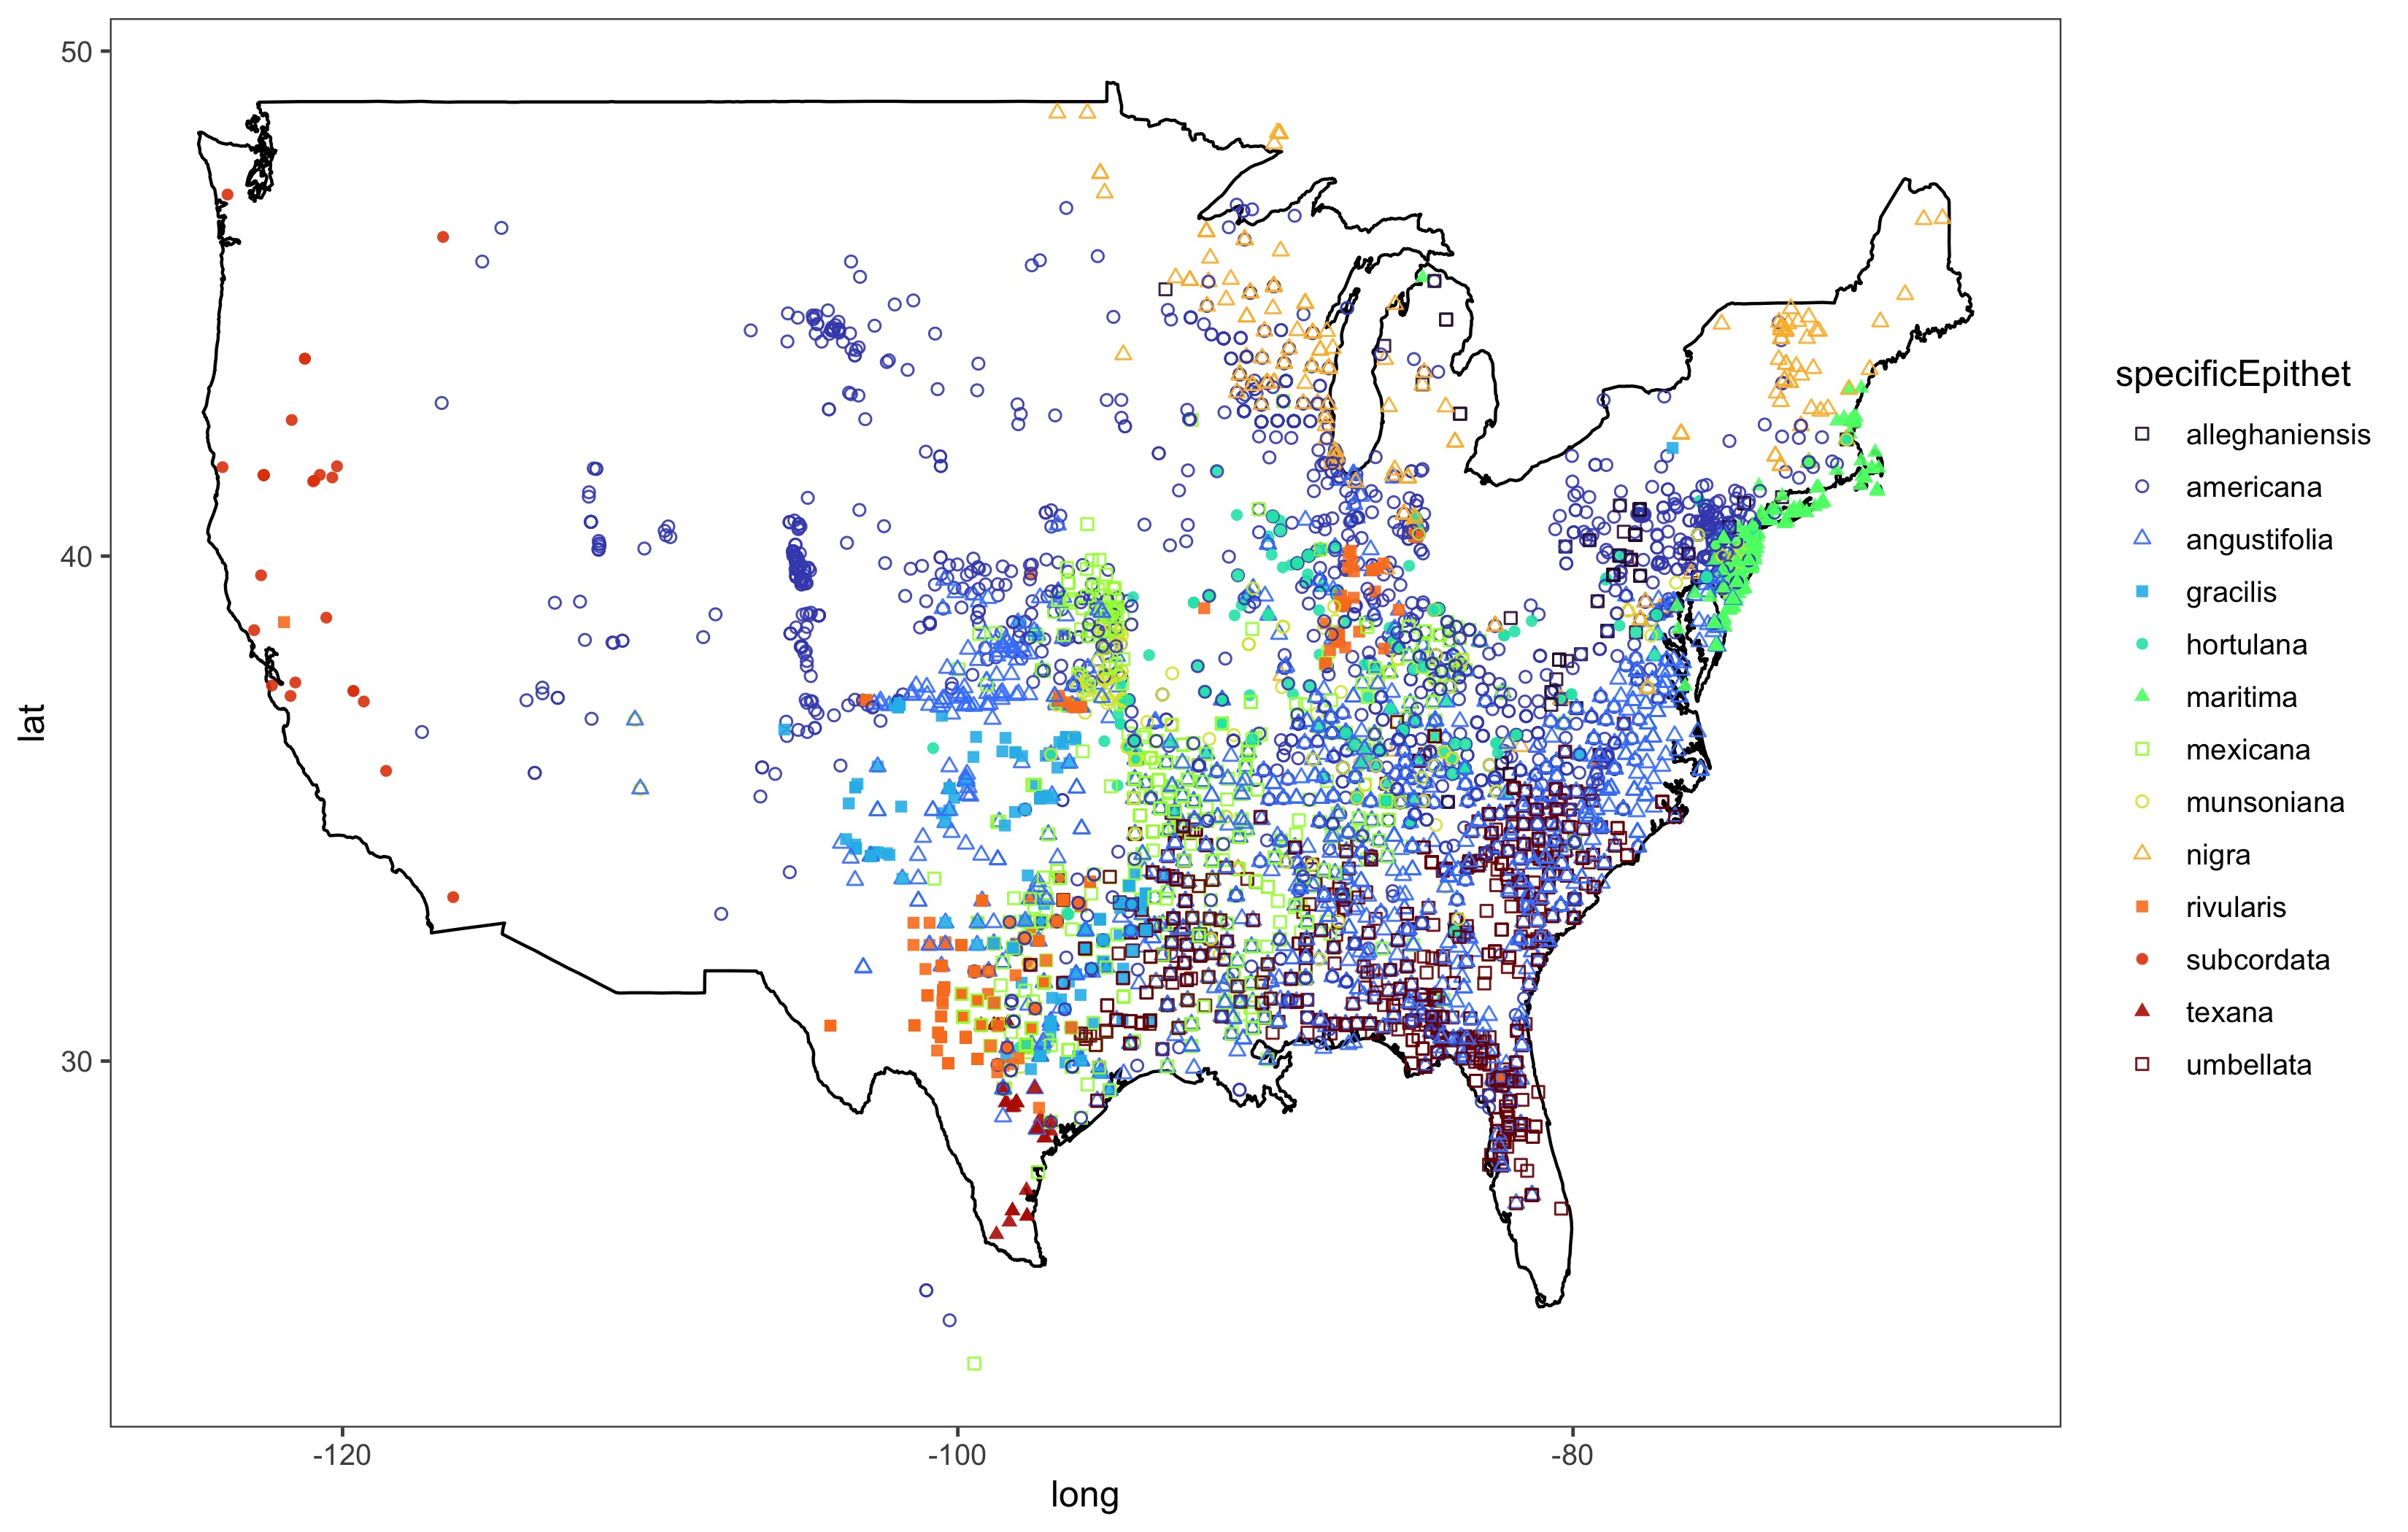
\includegraphics[width=\textwidth]{..//..//Plots/map.jpeg}
    \caption{Map to show where data come from and to point out the two never hysteranthy species are highly endemic}
    \label{fig:mappy}
\end{figure}

\begin{figure}[h!]
    \centering
 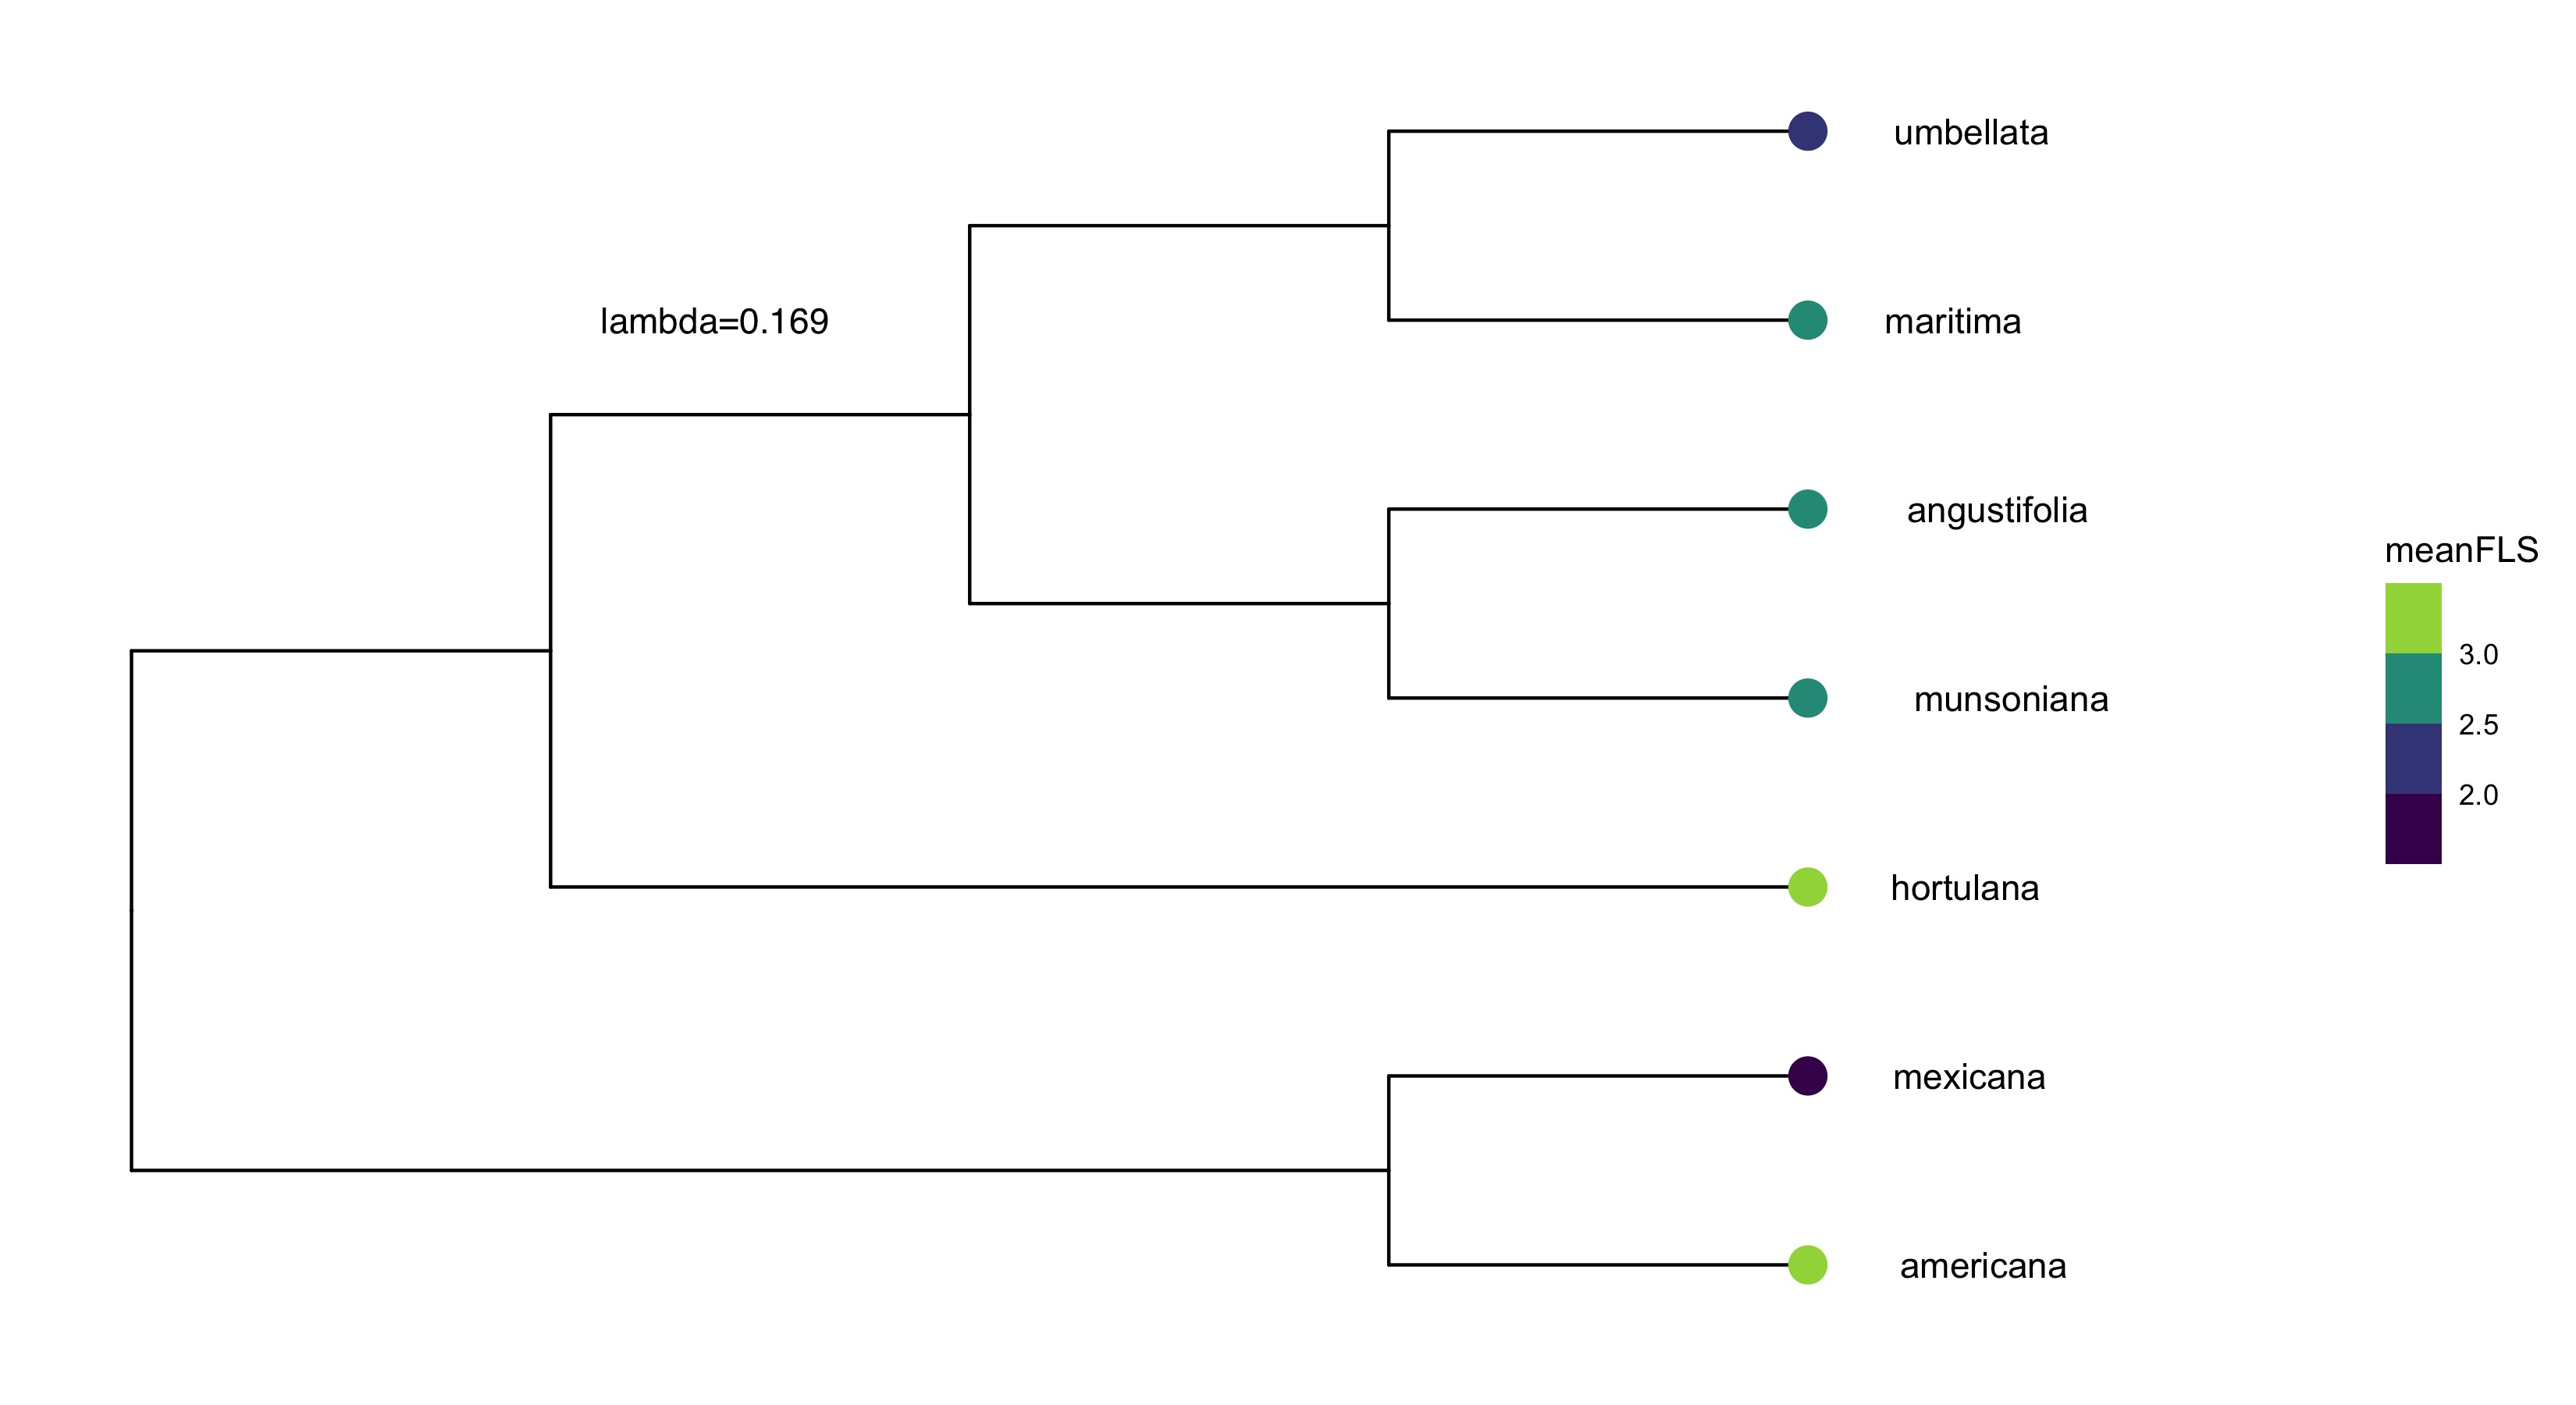
\includegraphics[width=\textwidth]{..//..//Plots/phylosig1.jpeg}
    \caption{place holder for the phylgenies: Ideally will have all N.A. Prunus \texit{and} Prunocerasus }
    \label{fig:phylo1}
\end{figure}

\begin{figure}[h!]
    \centering
 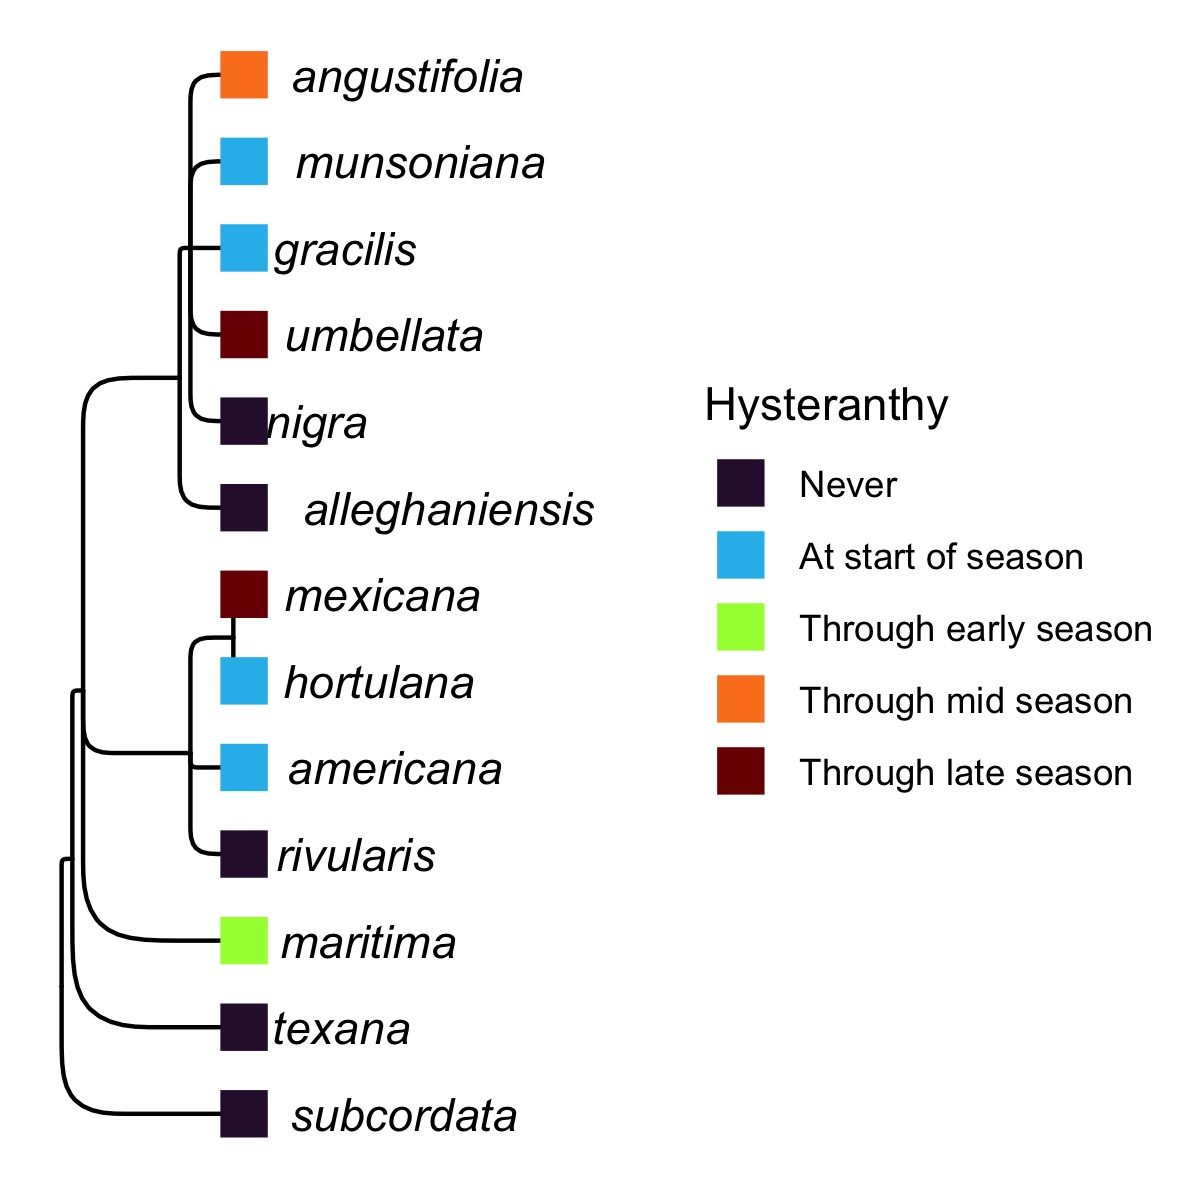
\includegraphics[width=\textwidth]{..//..//Plots/phylosig2.jpeg}
    \caption{place holder for the phylgenies: Ideally will have all N.A. Prunus \texit{and} Prunocerasus }
    \label{fig:phylo2}
\end{figure}

\begin{figure}[h!]
    \centering
 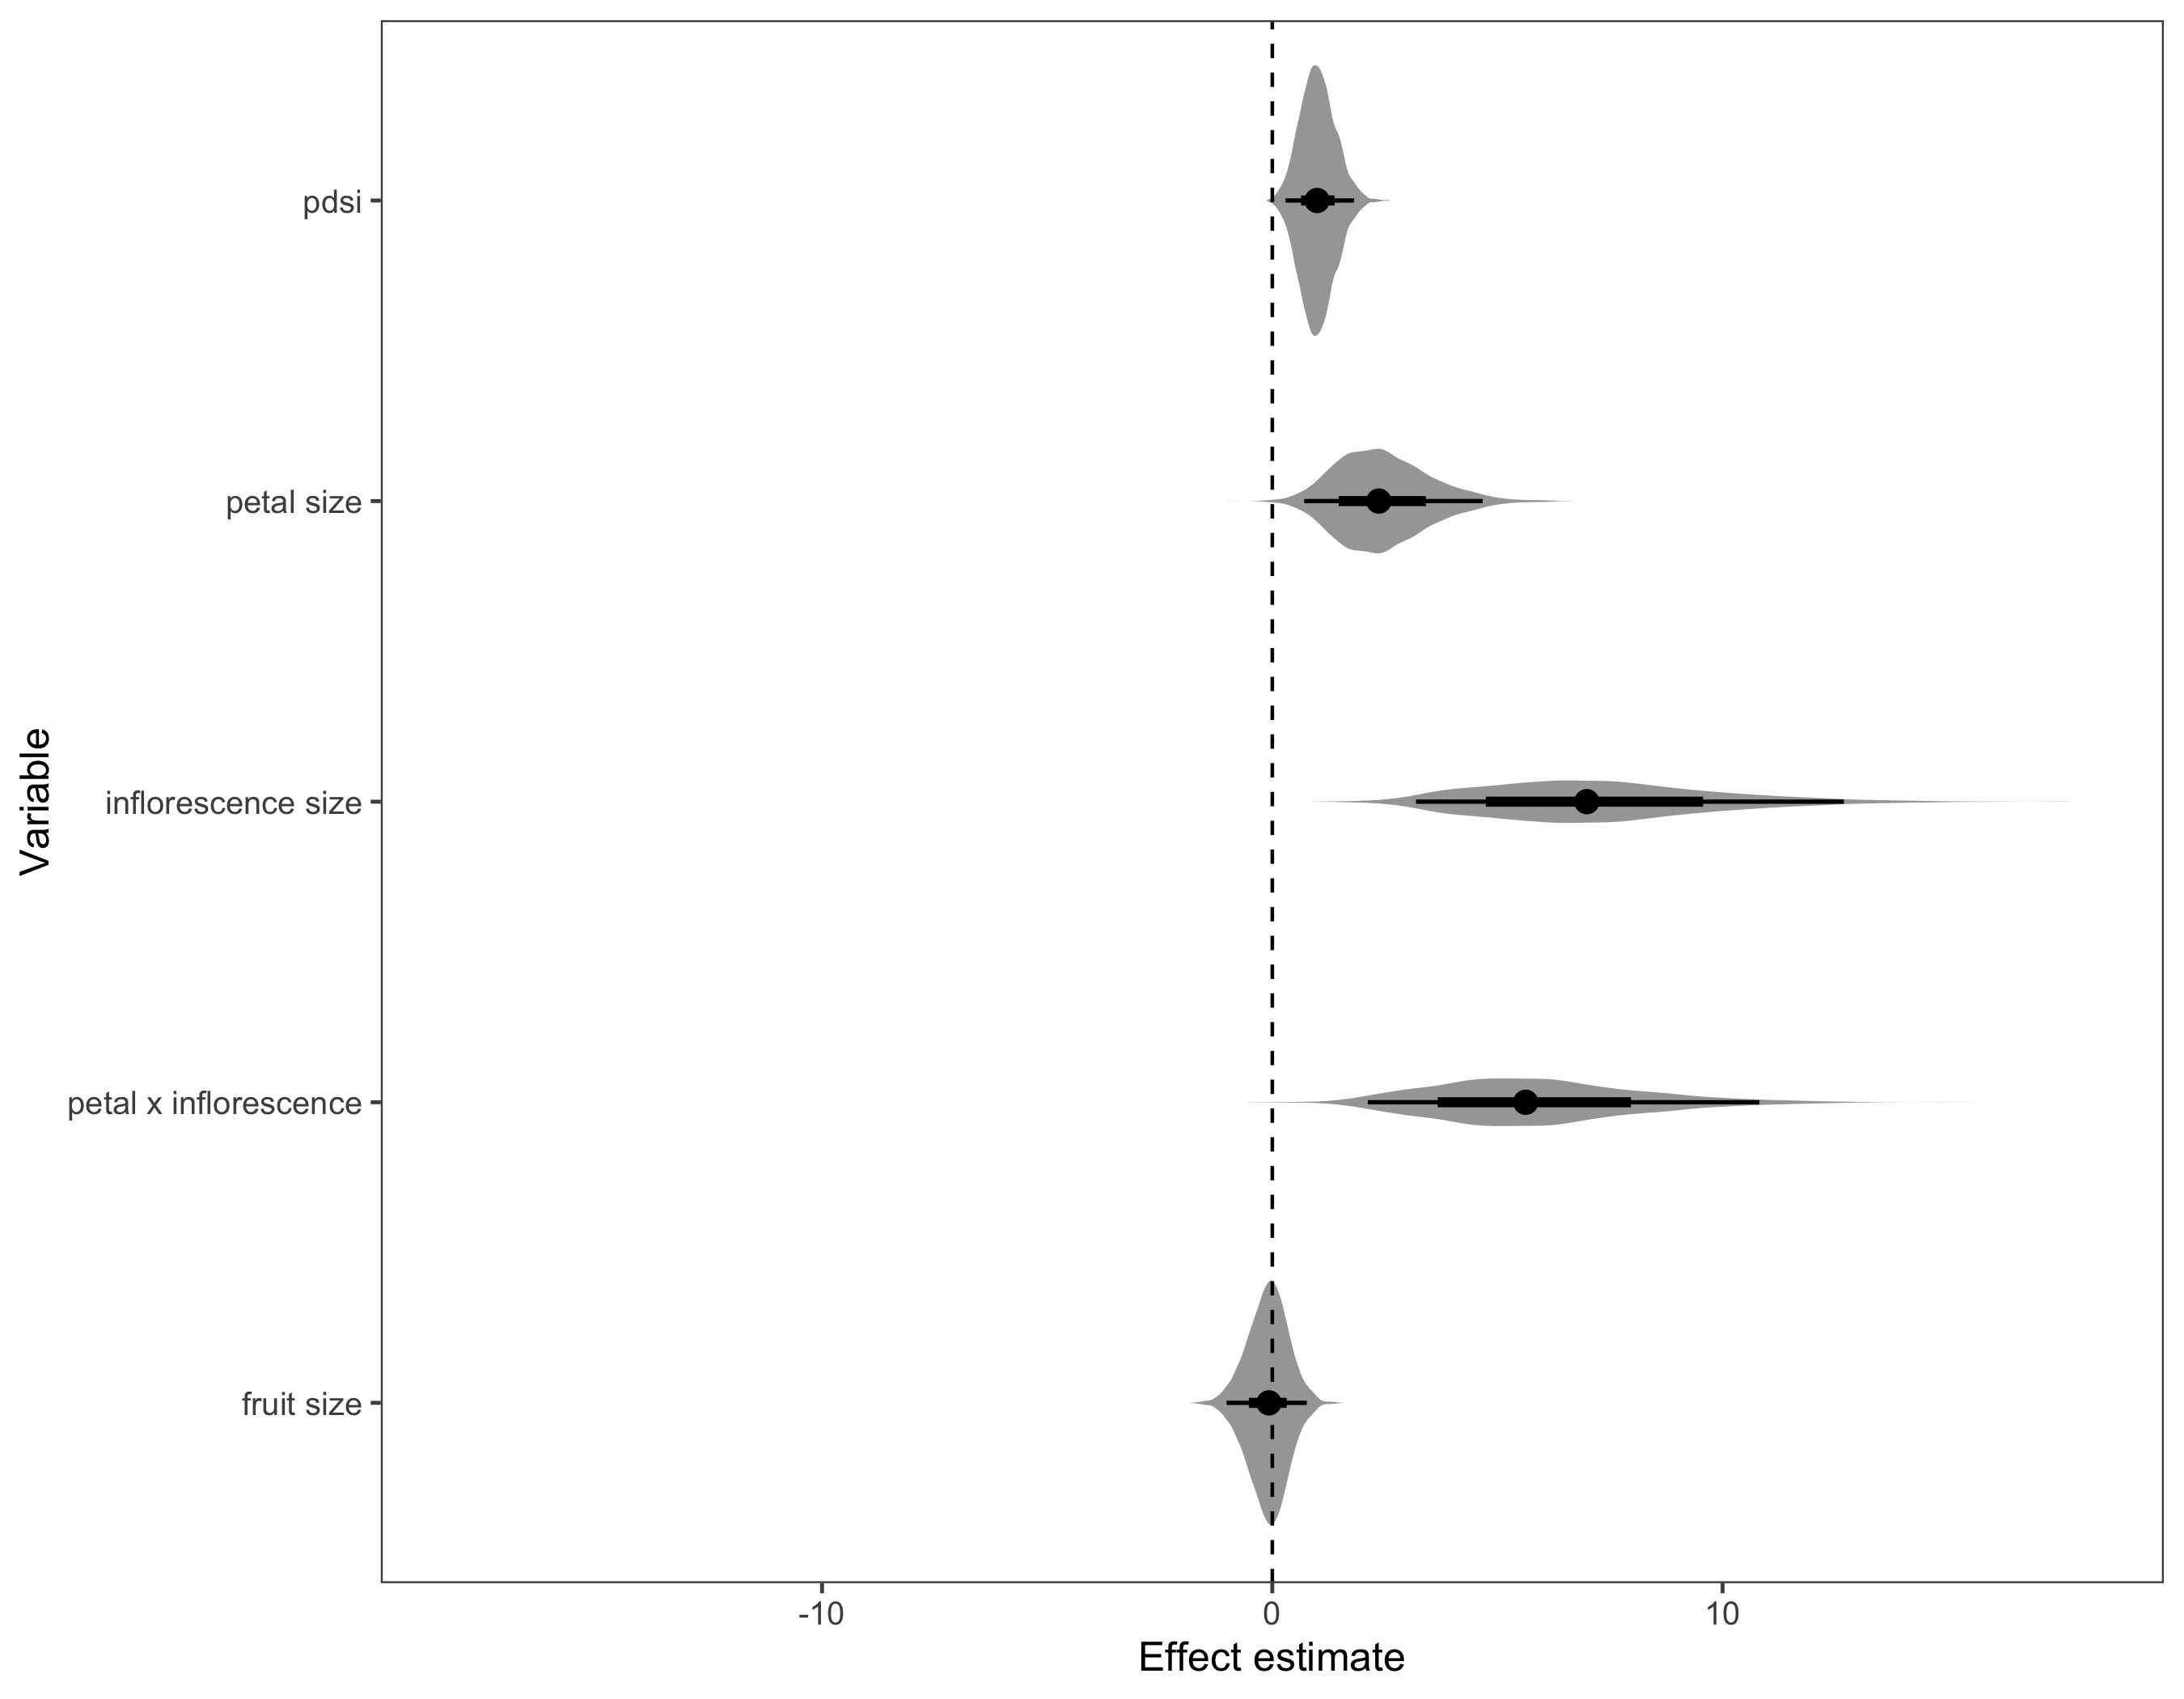
\includegraphics[width=\textwidth]{..//..//Plots/fullprunus_mus.jpeg}
    \caption{From the full genus analysis: Positive is less hysteranthus so aridity increases ihysteranthy, flower size decreases (ie smaller flowers- more hysteranthous) and no relationship with fruit size }
    \label{fig:cherries}
\end{figure}


\begin{figure}[h!]
    \centering
 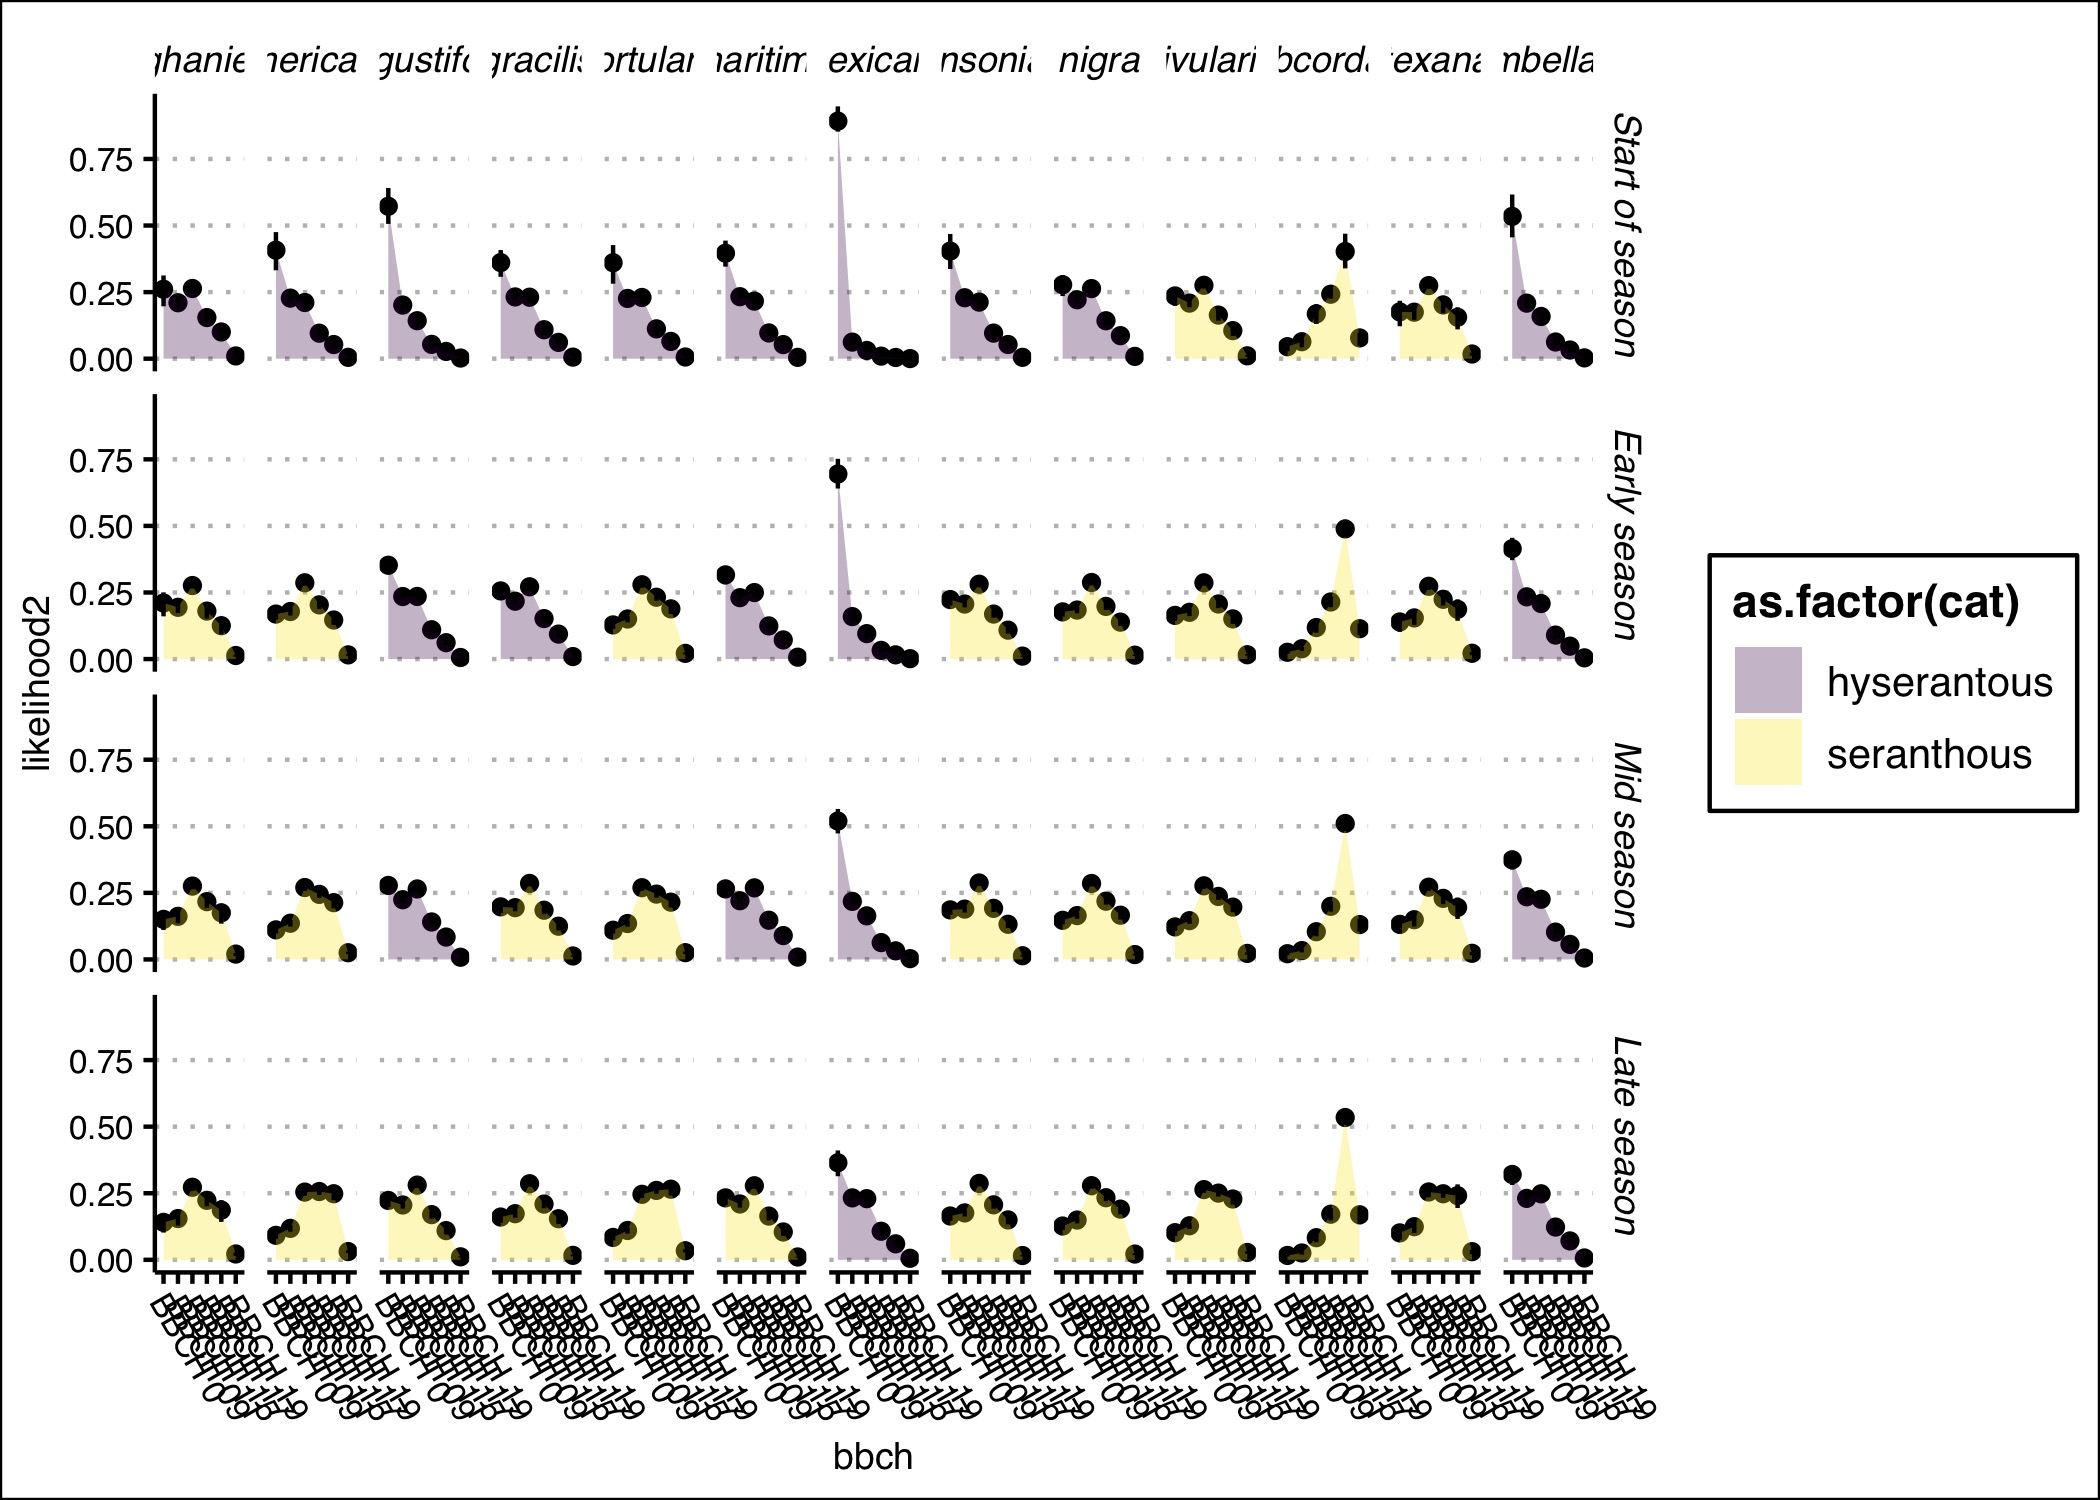
\includegraphics[width=\textwidth]{..//..//Plots/ord_quants.jpeg}
    \caption{ Likelihood of hysteranthy throughout the flowering season for each species in prunocerasus}
    \label{fig:plums}
\end{figure}

\begin{figure}[h!]
    \centering
 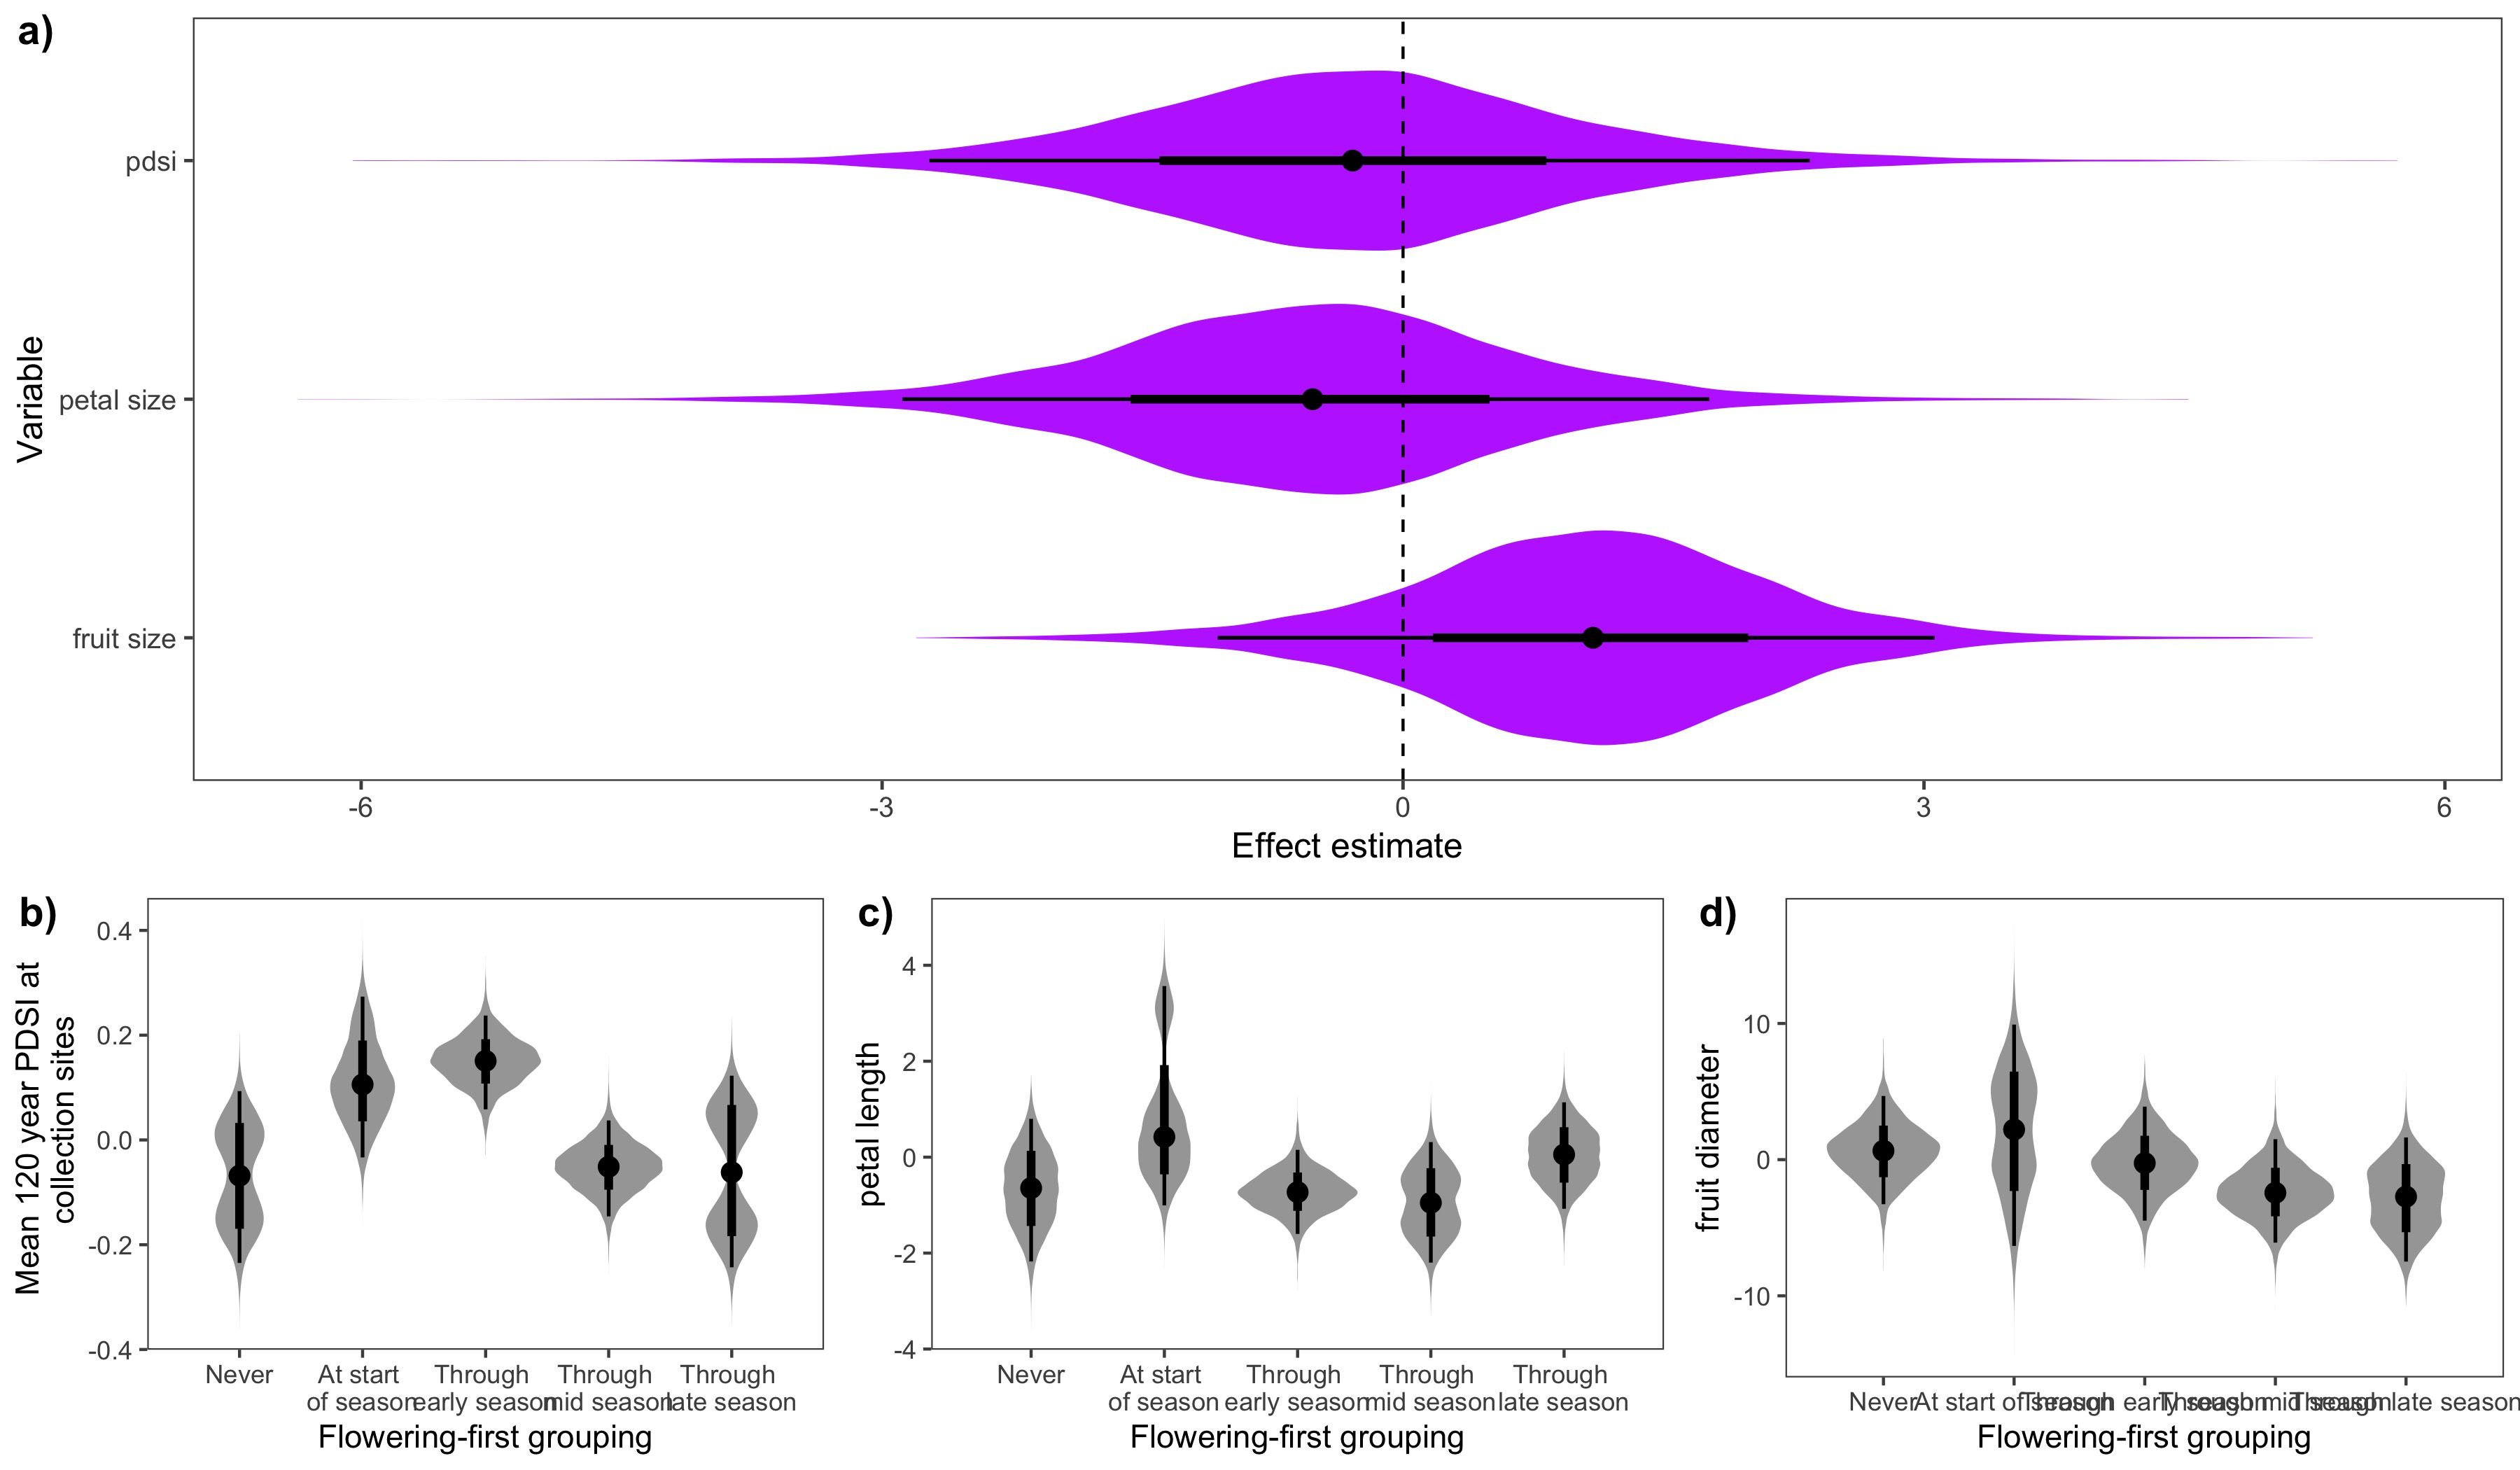
\includegraphics[width=\textwidth]{..//..//Plots/cerasus_mus.jpeg}
    \caption{Effect estimates. Why are they so different in prunucerasus? 1. measurement error model increases uncertainty. 2. outlyers have stronger influence. 3. Maybe too closely related (all flower to somedegree while leave are developing) }
    \label{fig:prunes}
\end{figure}


\begin{figure}[h!]
    \centering
 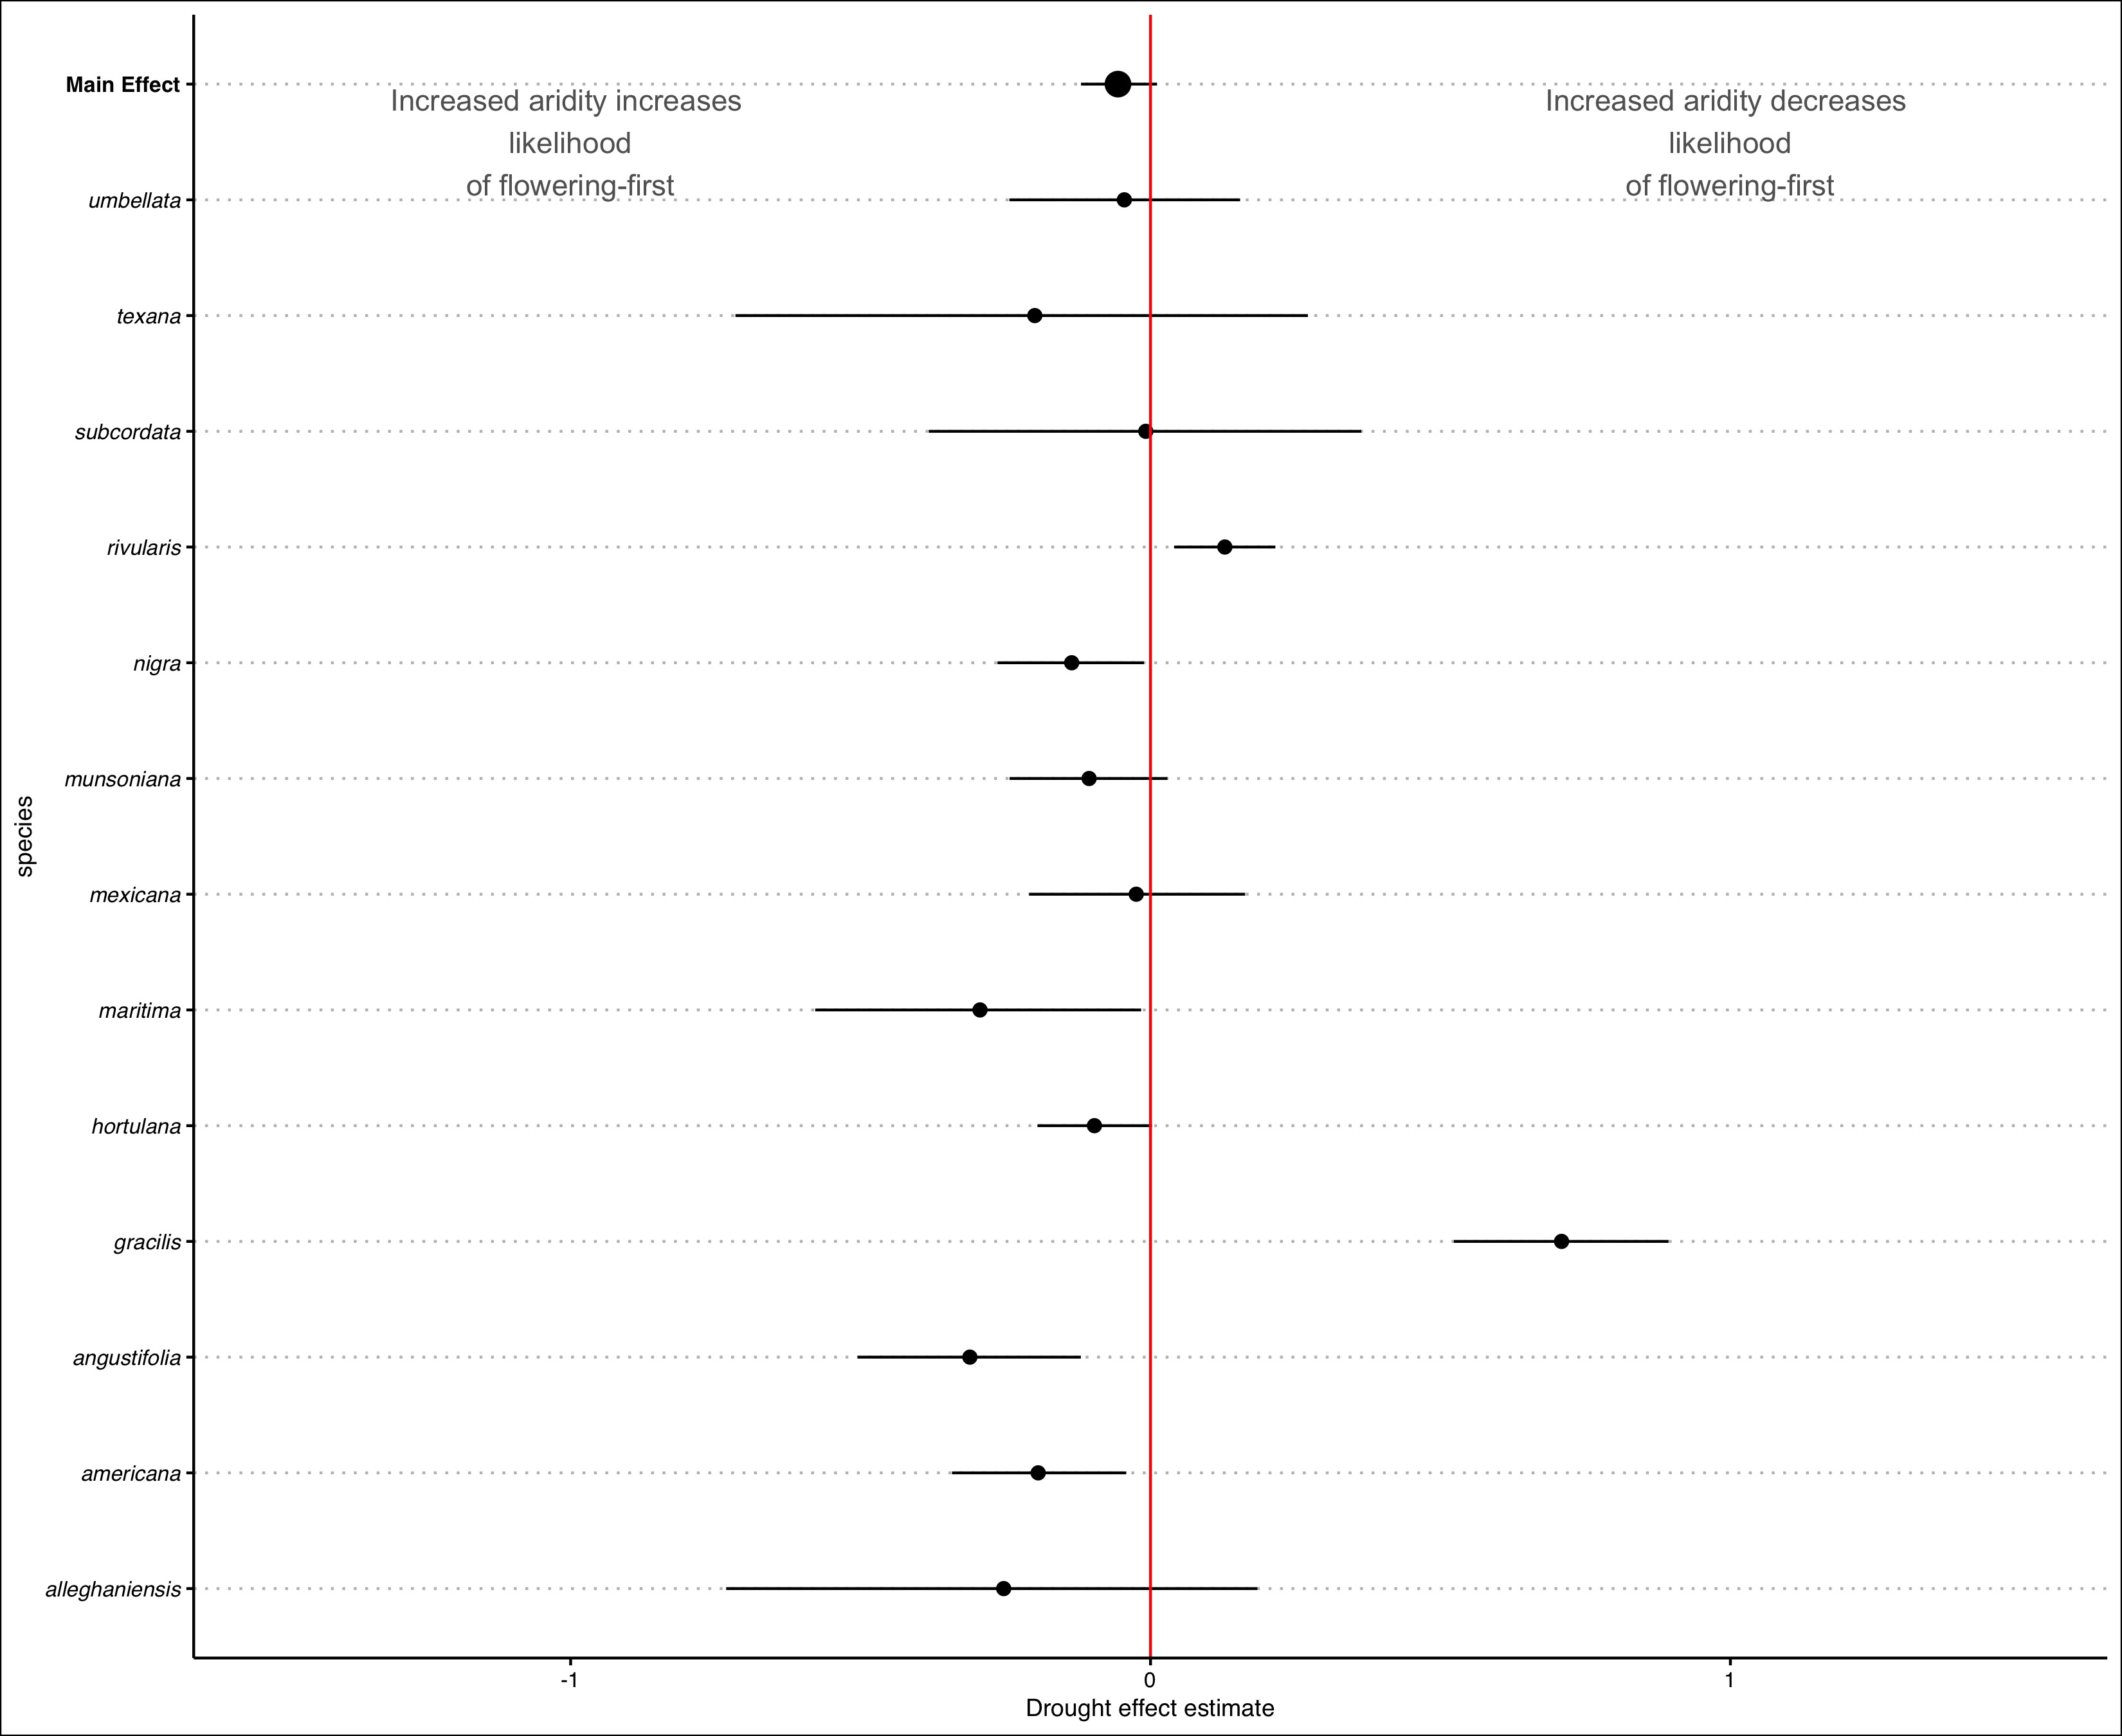
\includegraphics[width=\textwidth]{..//..//Plots/droughtstuff.jpg}
    \caption{Hysteranthy more likely in drought years.}
    \label{fig:plastic}
\end{figure}

\end{document}
